\chapter{Pattern Mining}
\section{Basket Construction}
Association-rule mining looks for implications between flags describing an account's behaviour before a loan. The pattern-mining script converts each account's pre-loan transactions into a basket of items: transaction type flags, high-amount activity, negative-balance behaviour, and the observed default outcome. Only transactions strictly before the loan date enter a basket, so the rules obey the same leakage boundary as the supervised features.

\section{Algorithms}
Two algorithms are run over the same baskets:
\begin{itemize}
    \item \textbf{Apriori}, a level-wise candidate-generation method that extends frequent itemsets one item at a time and prunes candidates whose subsets are not frequent.
    \item \textbf{FP-Growth}, which compresses the transactions into a frequent-pattern tree and mines it without generating candidate itemsets.
\end{itemize}

Both are run with minimum support $0.03$ and maximum itemset length $3$. They return the same 41 frequent itemsets, which is a useful consistency check between two different search strategies. The process is summarised in Figure~\ref{fig:pattern_flow}.

\begin{figure}[H]
    \centering
    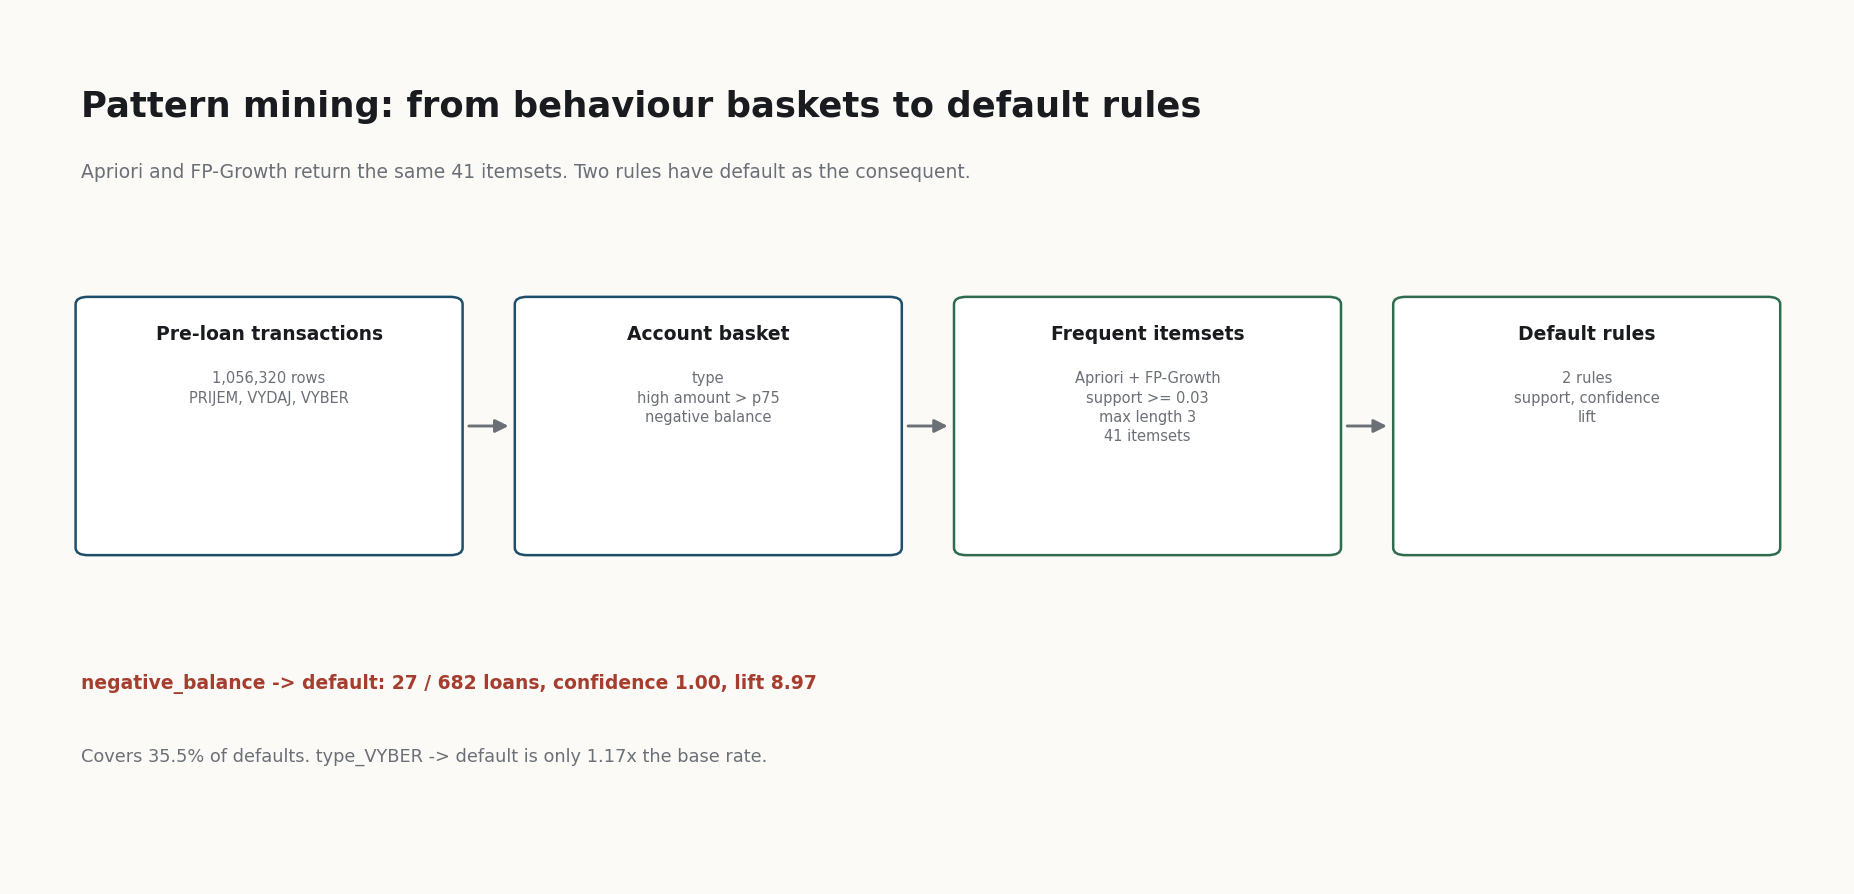
\includegraphics[width=0.88\textwidth]{figures/12_pattern_mining_flow.png}
    \caption{Pattern-mining pipeline from pre-loan baskets to default rules}
    \label{fig:pattern_flow}
\end{figure}

\section{Rules}
Rules are ranked by lift, which measures how much more often the consequent occurs with the antecedent than would be expected from the base rate. Two default-oriented rules survive the support threshold:

\begin{table}[H]
    \centering
    \small
    \renewcommand{\arraystretch}{1.25}
    \begin{tabular}{|l|c|c|c|}
        \hline
        \textbf{Rule} & \textbf{Support} & \textbf{Confidence} & \textbf{Lift} \\
        \hline
        \texttt{negative\_balance $\rightarrow$ default} & 0.0396 (27/682) & 1.000 & 8.97 \\
        \texttt{type\_VYBER $\rightarrow$ default} & 0.0704 (48/682) & 0.130 & 1.17 \\
        \hline
    \end{tabular}
    \caption{Default-oriented association rules}
    \label{tab:rules}
\end{table}

The negative-balance rule covers all 27 loans whose minimum pre-loan balance was negative, all of which defaulted. That is 35.5\% of the 76 defaults, with a lift of 8.97 over the 11.1\% base rate. It is the strongest single finding in the project and agrees with the supervised feature importance, where minimum balance is also the leading input.

The cash-withdrawal rule is only slightly above the base rate, so it is not a useful standalone screen. Its presence mainly confirms that high activity alone does not imply risk.

\section{Interpretation}
The rules are descriptive, not causal. A negative balance does not cause default, but it identifies a group with a much higher observed default rate. In practice the rule can be used as a transparent complement to the model score: a loan that satisfies the negative-balance rule deserves review even if its model score is moderate. The Patterns page of the dashboard shows the rules, itemset support, and rule coverage with covered-loan counts.
